% =============================================================================
%  SIMULACIÓN DE SISTEMAS - TP3
%  Grupo 05 - Sebastián Caules, Jerónimo Esquivel, Andrés Cortese
%  Sistema 1: Scanning rate en recinto cerrado con obstáculo fijo
%  Dinámica Molecular Regida por Eventos (EDMD)
% =============================================================================

\documentclass[10pt,aspectratio=169]{beamer}

\usetheme{Warsaw}
\usecolortheme{default}
\setbeamertemplate{navigation symbols}{}

% Header: miniframes con puntos de progreso por sección
\useoutertheme{miniframes}

% Footer: solo número de diapositiva a la derecha (igual al TP2)
\setbeamertemplate{footline}{%
    \hfill{\footnotesize\insertframenumber\,/\,\inserttotalframenumber}\hspace{8pt}\vspace{4pt}%
}

% Colores consistentes
\setbeamercolor{frametitle}{bg=blue!70!black, fg=white}

% --- Paquetes ---
\usepackage[utf8]{inputenc}
\usepackage[T1]{fontenc}
\usepackage[spanish]{babel}
\usepackage{amsmath,amssymb,amsfonts}
\usepackage{bm}
\usepackage{graphicx}
\usepackage{siunitx}
\usepackage{xcolor}
\usepackage{tikz}
\usetikzlibrary{arrows.meta,positioning,shapes.geometric,calc}
\usepackage{hyperref}

% Imagen representativa + link YouTube (versión entregable sin video embebido)
% Todos los videos: 1262×922 px
\newlength{\vidH}
\newlength{\vidW}
\newcommand{\simvideo}[2]{%   #1=N  #2=YouTube ID
  \setlength{\vidH}{0.55\textheight}%
  \pgfmathsetlength{\vidW}{\vidH * (1262/922)}%
  \parbox[c][\vidH][c]{\vidW}{\centering
    \includegraphics[width=\vidW,height=\vidH,keepaspectratio]{figures/N=#1.png}%
    \\[6pt]
    {\small\href{https://youtu.be/#2}{\texttt{youtu.be/#2}}}%
  }%
}

% Vectores: negrita sin itálica (punto 3.5)
\newcommand{\vect}[1]{\mathbf{#1}}

% --- Metadatos ---
\title[TP3 -- EDMD]{Scanning rate en recinto cerrado con obstáculo fijo}
\subtitle{Trabajo Práctico N\textsuperscript{o} 3}
\author[Caules, Esquivel, Cortese]{Sebastián Caules \and Jerónimo Esquivel \and Andrés Cortese}
\institute[ITBA]{Instituto Tecnológico de Buenos Aires \\ 72.25 -- Simulación de Sistemas -- Grupo 05}
\date{24 de abril de 2026}

\begin{document}

% =============================================================================
% PORTADA
% =============================================================================
    {
        \setbeamertemplate{headline}{}
        \setbeamertemplate{footline}{}
        \begin{frame}[plain]
  \titlepage
        \end{frame}
    }

% =============================================================================
% INTRODUCCIÓN
% FIX punto 4: texto corrido reemplazado por bullets cortos
% =============================================================================
    \section{Introducción}

    \begin{frame}[plain,c]
  \centering
  {\usebeamercolor[fg]{structure}\fontsize{48}{56}\selectfont Introducción\par}
    \end{frame}

    \begin{frame}{Sistema real y motivación}
        % FIX 4: eliminados párrafos corridos, reemplazados por bullets concisos
        \begin{itemize}
            \item Sistemas físicos modelables como partículas con interacciones por colisión: gases diluidos, granos, partículas brownianas.
            \item Sistema real simulado: glóblulos blancos del sistema inmunológico
        \end{itemize}
    \end{frame}

    \begin{frame}{Modelo matemático}
        % FIX 4: eliminado texto corrido; solo ecuaciones con descripción mínima
        % FIX 7: vectores en \mathbf{} (negrita sin itálica); escalares en itálica por defecto
        \begin{itemize}
            \item Entre colisiones: movimiento rectilíneo uniforme
            \[
                \vect{r}_i(t) = \vect{r}_i(t_0) + \vect{v}_i(t_0)\,(t - t_0).
            \]
            \item Colisión elástica entre partículas $i$ y $j$: impulso
            \[
                J = \frac{2\,m_i\,m_j\,(\Delta\vect{v}\cdot\Delta\vect{r})}{\sigma\,(m_i + m_j)},
                \qquad \sigma = r_i + r_j.
            \]
            \item Colisión con obstáculo fijo o borde: la componente normal invierte signo; la tangencial se conserva.
        \end{itemize}
    \end{frame}

% =============================================================================
%  SECCIÓN: IMPLEMENTACIÓN
% =============================================================================

    \section{Implementación}

    \begin{frame}[plain,c]
        \centering
        {\usebeamercolor[fg]{structure}\fontsize{48}{56}\selectfont Implementación\par}
    \end{frame}

    \begin{frame}{Arquitectura del proyecto}
        \begin{columns}[t]
            \column{0.55\textwidth}
            \textbf{Motor (Java)}
            \begin{itemize}
                \item \texttt{Simulator.java} — motor EDMD
                \item \texttt{Simulate.java} — batch runner
            \end{itemize}
            \vspace{0.3em}
            \textbf{Análisis}
            \begin{itemize}
                \item \texttt{SimulationAnalyzer.java} — $C_{fc}(t)$, $F_u(t)$, perfiles radiales
                \item \texttt{plotter.py} — figuras
            \end{itemize}
            \column{0.42\textwidth}
            \textbf{Visualización}
            \begin{itemize}
                \item \texttt{Visualizer.java} — animador Swing
            \end{itemize}
        \end{columns}
    \end{frame}

    \begin{frame}{Motor EDMD}
        \begin{enumerate}
            \item Inicializar $N$ partículas: posiciones en anillo $[r_0{+}r, R{-}r]$, velocidades $|\mathbf{v}| = v_0$
            \item Poblar cola con todos los eventos iniciales: $\mathcal{O}(N^2)$ pares PP + $N$ OBS + $N$ WALL
            \item \textbf{Mientras} $t < t_f$:
            \begin{enumerate}
                \item Extraer evento $e$ de mínimo tiempo
                \item Si contadores no coinciden: descartar \textit{(lazy deletion)}
                \item Avanzar todas las partículas $\Delta t = t_e - t$ \hfill $\mathcal{O}(N)$
                \item Aplicar operador de colisión; actualizar estado si corresponde
                \item Reprogramar eventos de partículas involucradas \hfill $\mathcal{O}(N \log N)$
            \end{enumerate}
        \end{enumerate}
    \end{frame}

    \begin{frame}{Flujo del proyecto}
        \begin{center}
            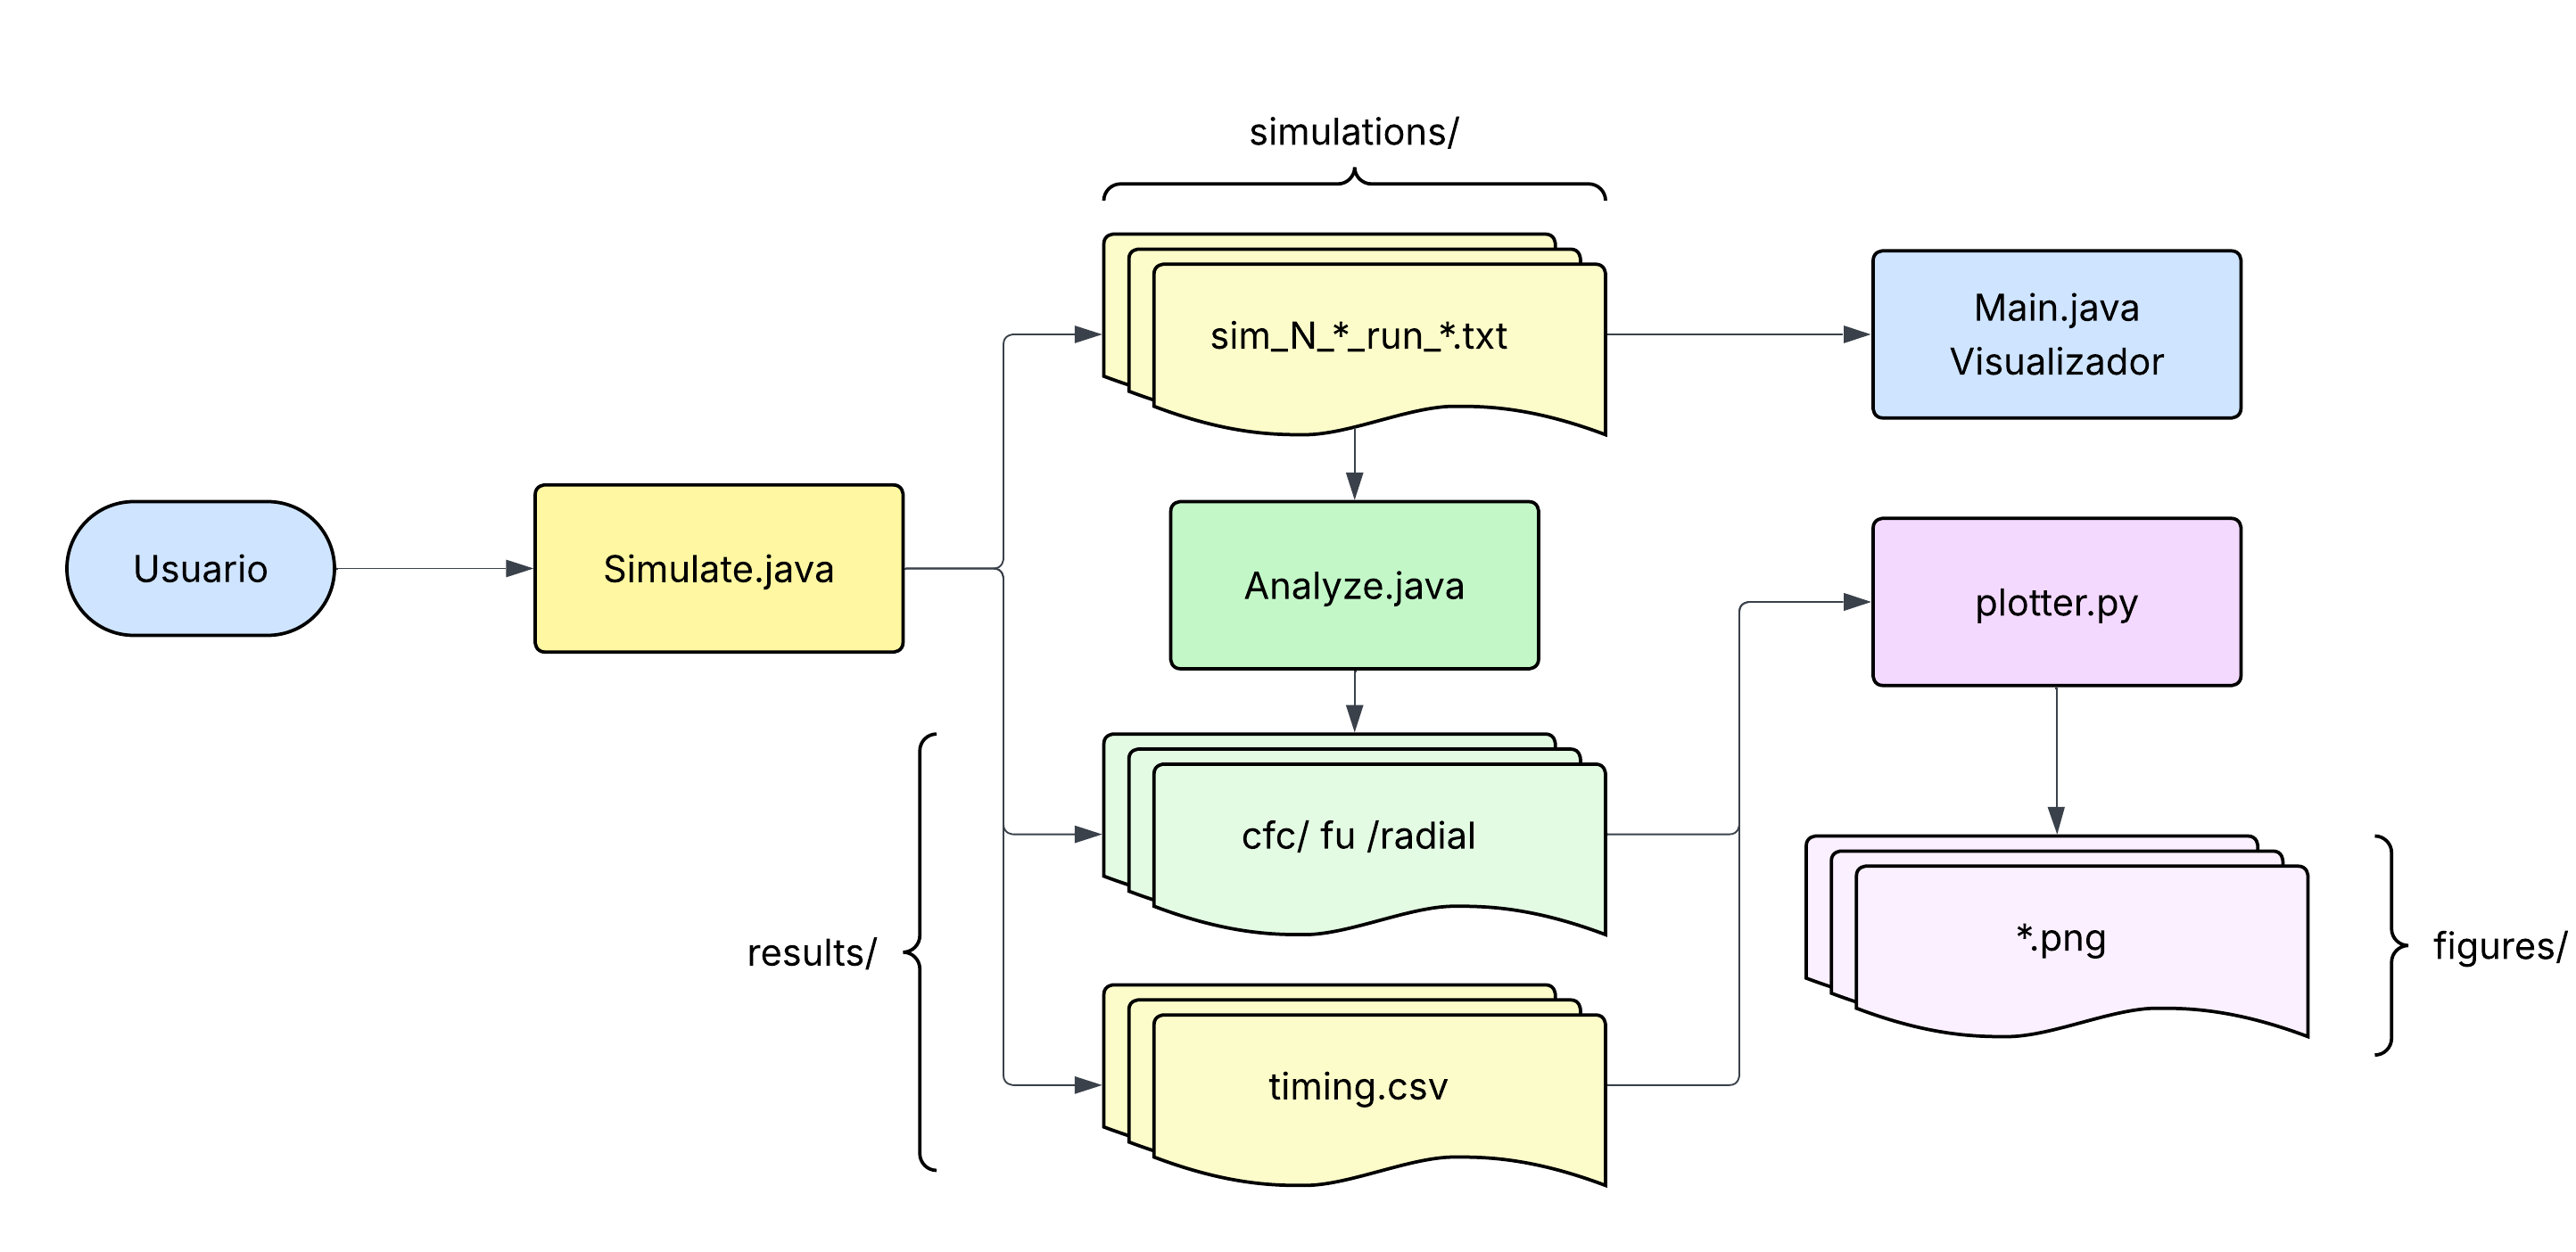
\includegraphics[width=0.92\textwidth]{figures/TP3_SDS.png}
        \end{center}
    \end{frame}


% =============================================================================
% SIMULACIONES
% FIX punto 7: vectores en negrita; escalares en itálica; unidades rectas
% =============================================================================
    \section{Simulaciones}

    \begin{frame}[plain,c]
  \centering
  {\usebeamercolor[fg]{structure}\fontsize{48}{56}\selectfont Simulaciones\par}
    \end{frame}

    \begin{frame}{Sistema particular}
        \begin{columns}[T]
            \begin{column}{0.55\textwidth}
                \begin{itemize}
                    \item Recinto circular de diámetro $L = \SI{80}{m}$.
                    \item Obstáculo fijo central, radio $r_0 = \SI{1}{m}$.
                    \item $N$ partículas de radio $r = \SI{1}{m}$, masa $m = \SI{1}{kg}$.
                    \item Velocidad inicial $v_0 = \SI{1}{m/s}$, dirección uniforme en $[0, 2\pi)$.
                    \item Colisiones elásticas: entre partículas, con obstáculo, con borde.
                    \item Distribución inicial uniforme, sin solapamiento.
                    \item Estados:
                    \begin{itemize}
                        \item \textcolor{green!55!black}{\textbf{Fresca}}: inicial; al tocar obstáculo $\to$ usada.
                        \item \textcolor{violet!70!black}{\textbf{Usada}}: al tocar borde $\to$ fresca.
                    \end{itemize}
                \end{itemize}
            \end{column}
            \begin{column}{0.45\textwidth}
                \centering
                \begin{tikzpicture}[scale=0.85]
        \draw[thick] (0,0) circle (3);
        \fill[violet!70!black] (0,0) circle (0.25);
        \foreach \x/\y in {1.2/0.5, -1.5/0.8, 0.3/-1.8, 1.8/-1.2, -0.9/-2.1, -2.0/-0.4, 0.7/2.1, 1.9/1.5}
        \fill[green!60!black] (\x,\y) circle (0.12);
        \foreach \x/\y in {-0.5/1.6, 2.2/0.3, -1.8/1.8}
        \fill[violet!70!black] (\x,\y) circle (0.12);
        \draw[<->] (-3,-3.4) -- (3,-3.4) node[midway,below,font=\small]{$L$};
        \node[font=\scriptsize] at (0.5,0.15) {$r_0$};
                \end{tikzpicture}
            \end{column}
        \end{columns}
    \end{frame}

    \begin{frame}{Observables (I): Conteo de cambio de estado y scanning rate}
        \textbf{Conteo acumulado de cambios de estado:}
        \[
            C_{fc}(t) = \#\{\text{transiciones fresca}\to\text{usada en }[0,t]\}.
        \]

        \textbf{Scanning rate} (pendiente en régimen estacionario):
        \[
            J = \left.\frac{\mathrm{d}\,C_{fc}(t)}{\mathrm{d}\,t}\right|_{\text{estacionario}}.
        \]
    \end{frame}

    \begin{frame}{Observables (II): Fracción de partículas usadas}
        \textbf{Observable transitorio:}
        \[
            F_u(t) = \frac{N_u(t)}{N}.
        \]

        \textbf{Observable estacionario:} $F_{\text{est}}(N)$, valor asintótico de $F_u(t)$.
    \end{frame}

    \begin{frame}{Observables (III): perfiles radiales}
        % FIX 7: \vect{R}_j, \vect{v}_j en negrita; S, t escalares en itálica
        Capas concéntricas de ancho $\mathrm{d}S = \SI{0.2}{m}$.
        Partículas frescas entrantes $P_f^{\,\text{in}}$: $\vect{R}_j\cdot\vect{v}_j < 0$.

        \vspace{0.15cm}
        \textbf{Densidad promedio:}
        \[
            \langle\rho_f^{\,\text{in}}\rangle(S) =
            \frac{1}{M\,T}\sum_{k=1}^{M}\sum_{t\in T_k}
            \frac{n_k^{\,\text{in}}(S,t)}{A(S)},
            \quad A(S) = \pi\!\left[\!\left(S+\tfrac{\mathrm{d}S}{2}\right)^{\!2}-\left(S-\tfrac{\mathrm{d}S}{2}\right)^{\!2}\right].
        \]

        \textbf{Velocidad normal promedio:}
        \[
            \langle v_f^{\,\text{in}}\rangle(S) =
            \frac{1}{M\,T}\sum_{k,t} \frac{1}{n_k^{\,\text{in}}(S,t)}
            \sum_{j\in P_f^{\,\text{in}}(S,t)} \frac{\vect{R}_j\cdot\vect{v}_j}{|\vect{R}_j|}.
        \]

        \textbf{Flujo radial entrante:}
        $J_{\text{in}}(S) = \langle\rho_f^{\,\text{in}}\rangle(S)\,|\langle v_f^{\,\text{in}}\rangle(S)|$.
    \end{frame}

    \begin{frame}{Parámetros y realizaciones}
        \textbf{Parámetros variables}
        \begin{itemize}
            \item $N \in \{10, 50, 100, 200, 400, 800\}$.
            \item $t_f = \SI{500}{s}$ (tiempos de ejecución); $t_f = \SI{2500}{s}$ (puntos 1.2--1.4).
        \end{itemize}

        \vspace{0.3cm}
        \textbf{Realizaciones:}
        \begin{itemize}
            \item $M = 10$ (tiempos de ejecución); $M = 5$ (puntos 1.2--1.4).
            \item Modo Light para $N \geq 400$: snapshot cada 1000 eventos.
        \end{itemize}
    \end{frame}

% =============================================================================
% RESULTADOS
% FIX punto 5: captions debajo de figuras eliminados; info movida al costado
% =============================================================================
    \section{Resultados}

    \begin{frame}[plain,c]
  \centering
  {\usebeamercolor[fg]{structure}\fontsize{48}{56}\selectfont Resultados\par}
    \end{frame}


    \begin{frame}{$N = 10$}
        \begin{columns}[T]
            \begin{column}{0.65\textwidth}
                \centering
                \simvideo{10}{gh6J099zjYc}
            \end{column}
            \begin{column}{0.35\textwidth}
                \textbf{Condiciones}
                \begin{itemize}
                    \item $N = 10$
                    \item $t_f = \SI{2500}{s}$
                \end{itemize}
            \end{column}
        \end{columns}
    \end{frame}

    \begin{frame}{$N = 50$}
        \begin{columns}[T]
            \begin{column}{0.65\textwidth}
                \centering
                \simvideo{50}{cN-FYxtJ3wg}
            \end{column}
            \begin{column}{0.35\textwidth}
                \textbf{Condiciones}
                \begin{itemize}
                    \item $N = 50$
                    \item $t_f = \SI{2500}{s}$
                \end{itemize}
            \end{column}
        \end{columns}
    \end{frame}

    \begin{frame}{$N = 100$}
        \begin{columns}[T]
            \begin{column}{0.65\textwidth}
                \centering
                \simvideo{100}{xxuA8FSFT3o}
            \end{column}
            \begin{column}{0.35\textwidth}
                \textbf{Condiciones}
                \begin{itemize}
                    \item $N = 100$
                    \item $t_f = \SI{2500}{s}$
                \end{itemize}
            \end{column}
        \end{columns}
    \end{frame}

    \begin{frame}{$N = 200$}
        \begin{columns}[T]
            \begin{column}{0.65\textwidth}
                \centering
                \simvideo{200}{bNDo_GcceHc}
            \end{column}
            \begin{column}{0.35\textwidth}
                \textbf{Condiciones}
                \begin{itemize}
                    \item $N = 200$
                    \item $t_f = \SI{2500}{s}$
                \end{itemize}
            \end{column}
        \end{columns}
    \end{frame}

    \begin{frame}{$N = 400$}
        \begin{columns}[T]
            \begin{column}{0.65\textwidth}
                \centering
                \simvideo{400}{Fg7fypwaZWA}
            \end{column}
            \begin{column}{0.35\textwidth}
                \textbf{Condiciones}
                \begin{itemize}
                    \item $N = 400$
                    \item $t_f = \SI{2500}{s}$
                    \item Modo Light activo
                \end{itemize}
            \end{column}
        \end{columns}
    \end{frame}

    \begin{frame}{$N = 800$}
        \begin{columns}[T]
            \begin{column}{0.65\textwidth}
                \centering
                \simvideo{800}{S9UglmROl6Y}
            \end{column}
            \begin{column}{0.35\textwidth}
                \textbf{Condiciones}
                \begin{itemize}
                    \item $N = 800$
                    \item $t_f = \SI{2500}{s}$
                    \item Modo Light activo
                \end{itemize}
            \end{column}
        \end{columns}
    \end{frame}

% -----------------------------------------------------------------------------
% 1.1) Tiempo de ejecución
% -----------------------------------------------------------------------------

    \begin{frame}{Tiempo de ejecución vs $N$}
        \begin{columns}[T]
            \begin{column}{0.65\textwidth}
                \centering
                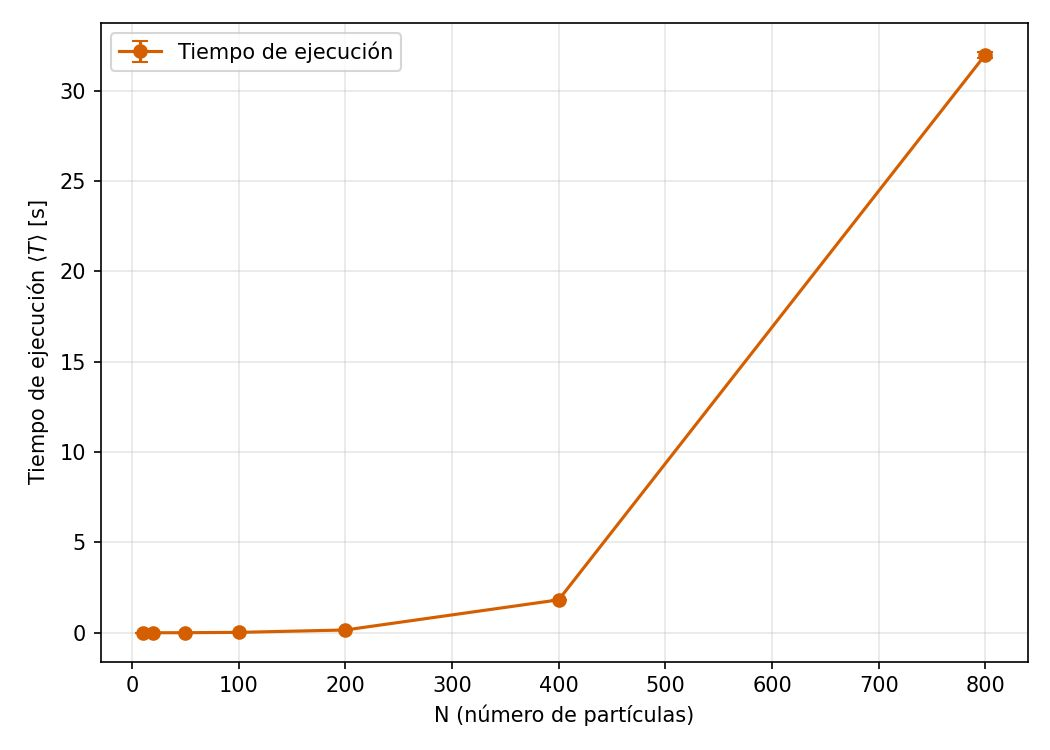
\includegraphics[width=\linewidth,height=5.5cm,keepaspectratio]{figures/graficos/1_1_tiempo_vs_N.jpeg}
            \end{column}
            \begin{column}{0.35\textwidth}
                \textbf{Condiciones}
                \begin{itemize}
                    \item $t_f = \SI{500}{s}$
                    \item $M = 10$ realizaciones
                \end{itemize}
                \vspace{0.3cm}
                \textbf{Observación}\\
                Crecimiento exponencial con $N$.
            \end{column}
        \end{columns}
    \end{frame}

    \begin{frame}{$\log(t_{\text{ejec}})$ vs $\log(N)$}
        \begin{columns}[T]
            \begin{column}{0.65\textwidth}
                \centering
                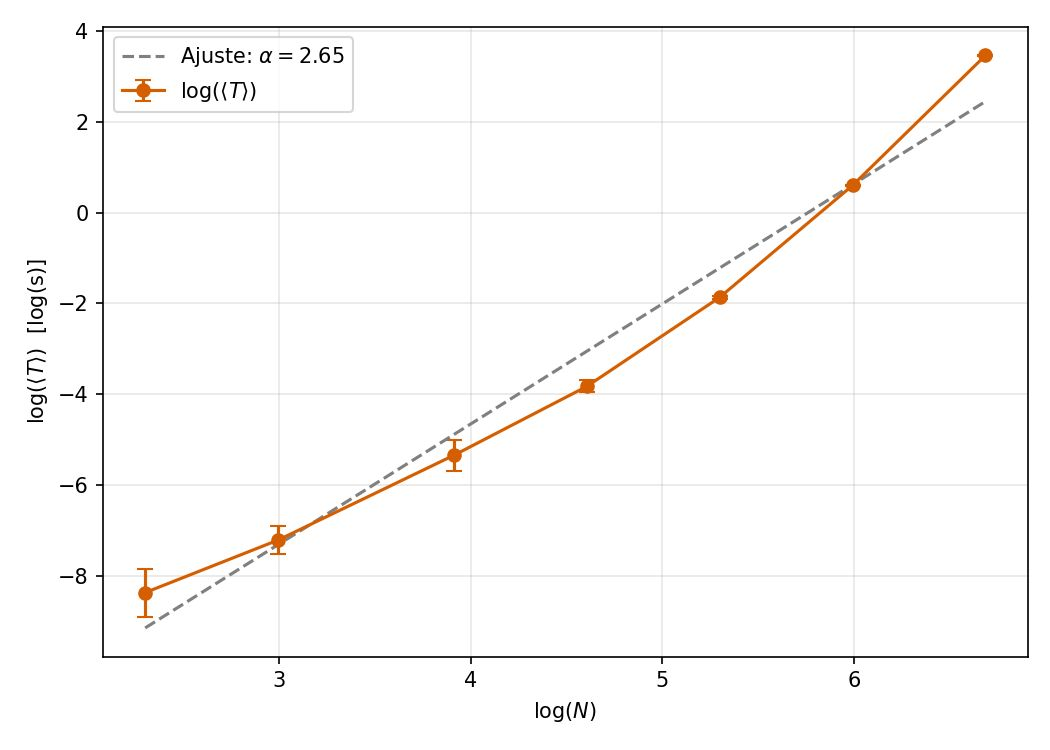
\includegraphics[width=\linewidth,height=5.5cm,keepaspectratio]{figures/graficos/1_1_loglog_tiempo_vs_N.jpeg}
            \end{column}
            \begin{column}{0.35\textwidth}
                \textbf{Condiciones}
                \begin{itemize}
                    \item $t_f = \SI{500}{s}$
                    \item $M = 10$ realizaciones
                \end{itemize}
                \vspace{0.3cm}
                \textbf{Observación}\\
                Comportamiento quasi-lineal; ajuste conpendiente: $\alpha=2.65$.
            \end{column}
        \end{columns}
    \end{frame}

% -----------------------------------------------------------------------------
% 1.2) Scanning rate
% -----------------------------------------------------------------------------

    \begin{frame}{Evolución temporal de $C_{fc}(t)$}
        \begin{columns}[T]
            \begin{column}{0.65\textwidth}
                \centering
                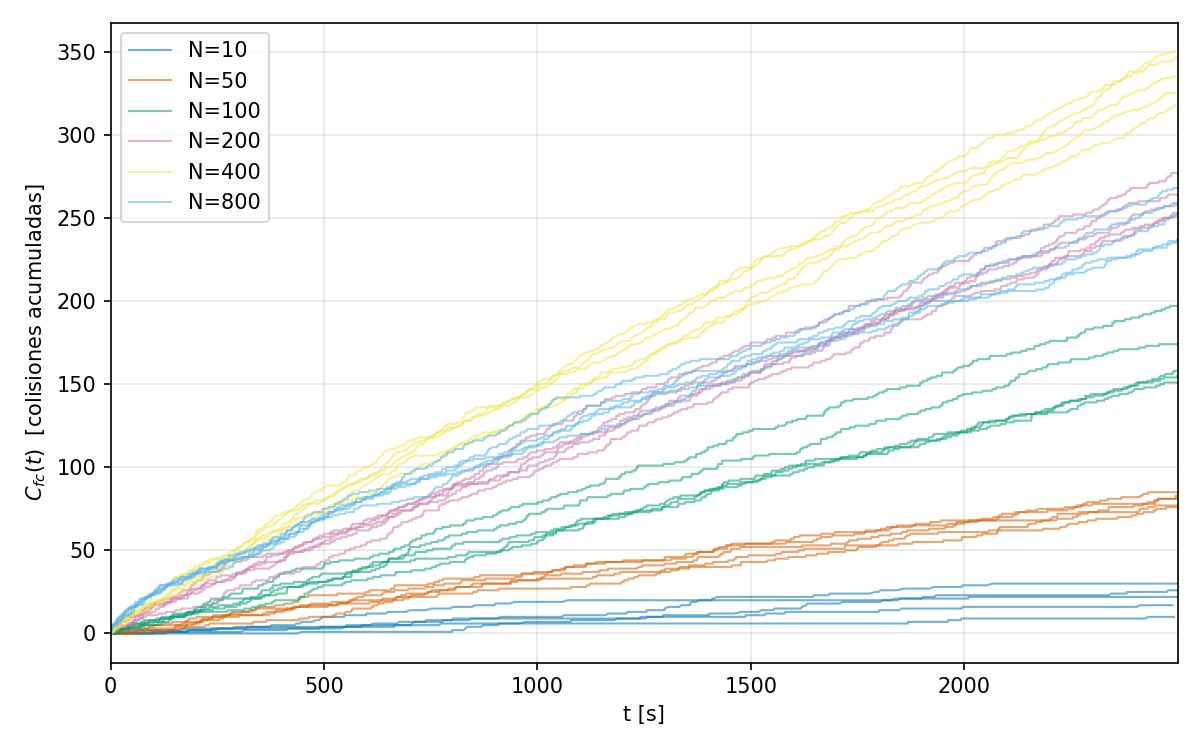
\includegraphics[width=\linewidth,height=5.5cm,keepaspectratio]{figures/graficos/1_2_Cfc_vs_t.jpeg}
            \end{column}
            \begin{column}{0.35\textwidth}
                \textbf{Observación}\\
                Régimen estacionario desde $t=0$ para todo $N$.
            \end{column}
        \end{columns}
    \end{frame}

    \begin{frame}{$\langle J\rangle$ en función de $N$}
        \begin{columns}[T]
            \begin{column}{0.65\textwidth}
                \centering
                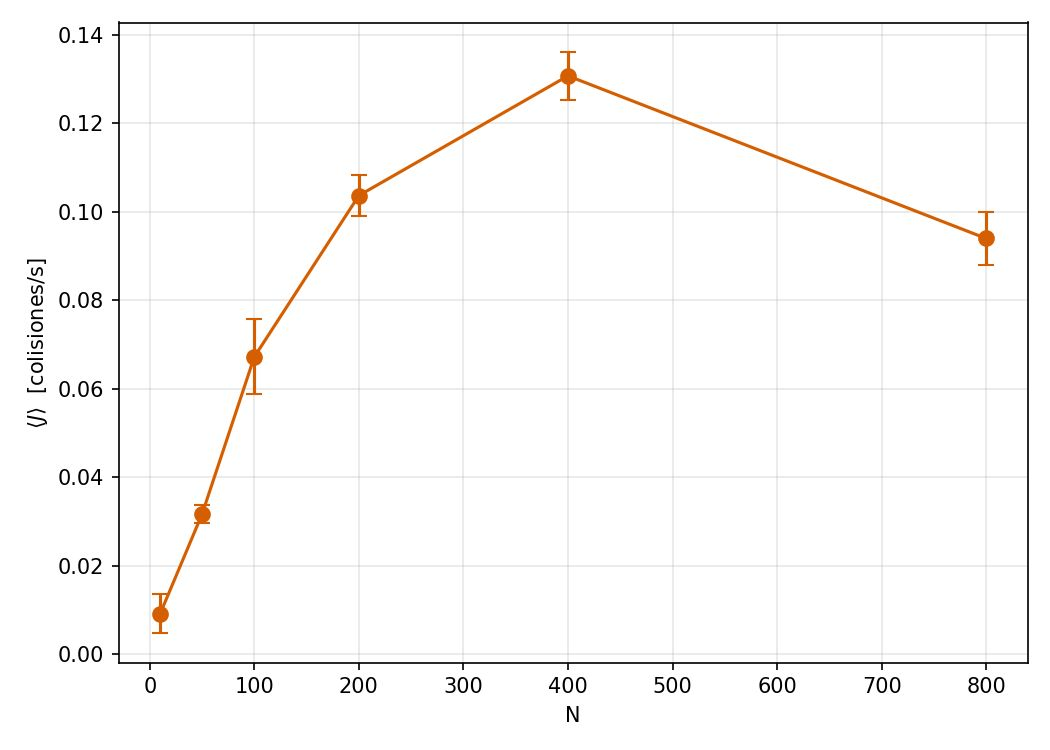
\includegraphics[width=\linewidth,height=5.5cm,keepaspectratio]{figures/graficos/1_2_J_vs_N.jpeg}
            \end{column}
            \begin{column}{0.35\textwidth}
                \textbf{Observación}\\
                Máximo en $N \approx 400$; para $N$ mayor las partículas usadas bloquean el acceso al obstáculo.
            \end{column}
        \end{columns}
    \end{frame}

% -----------------------------------------------------------------------------
% 1.3) Fracción de partículas usadas
% -----------------------------------------------------------------------------

    \begin{frame}{Evolución temporal de $F_u(t)$}
        \begin{columns}[T]
            \begin{column}{0.65\textwidth}
                \centering
                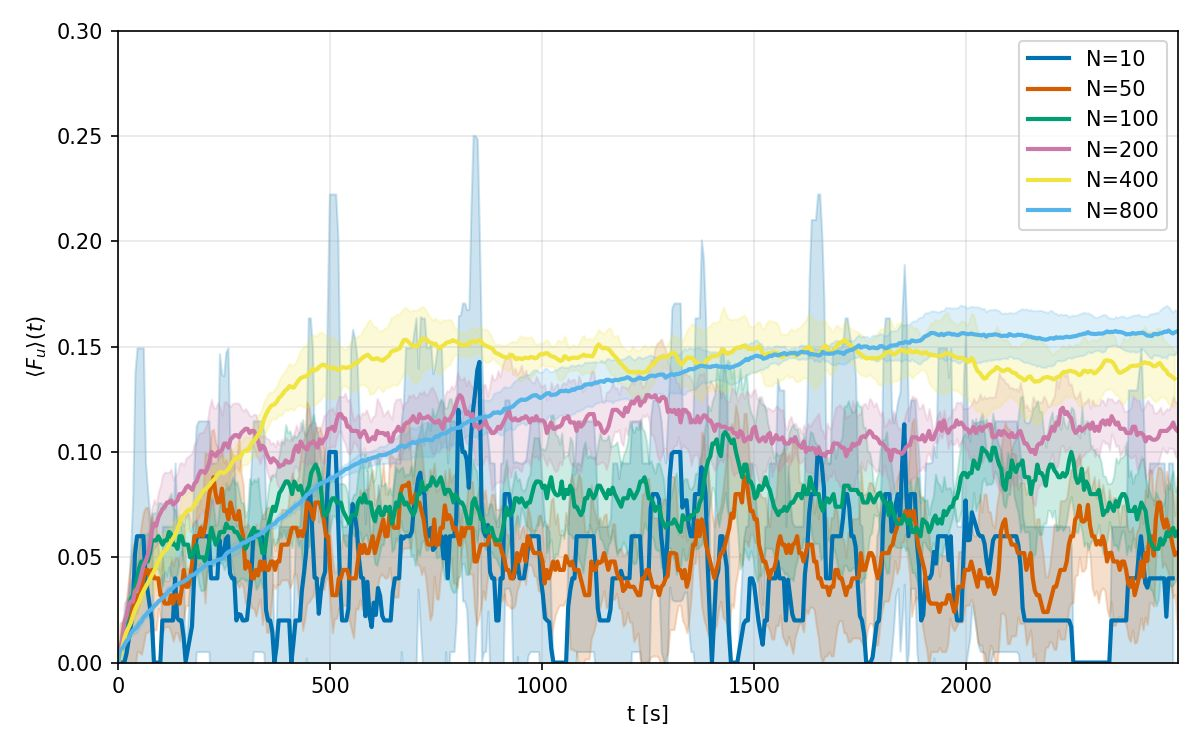
\includegraphics[width=\linewidth,height=5.5cm,keepaspectratio]{figures/graficos/1_3_Fu_promedio_vs_t.jpeg}
            \end{column}
            \begin{column}{0.35\textwidth}
                \textbf{Observaciones}
                \begin{itemize}
                    \item $N$ chico: estacionario rápido, alta variabilidad.
                    \item $N$ grande: estacionario tardío, menor variabilidad.
                \end{itemize}
            \end{column}
        \end{columns}
    \end{frame}

    \begin{frame}{$F_{\text{est}}$ y $t_{\text{est}}$ en función de $N$}
        \begin{columns}[T]
            \begin{column}{0.5\textwidth}
                \centering
                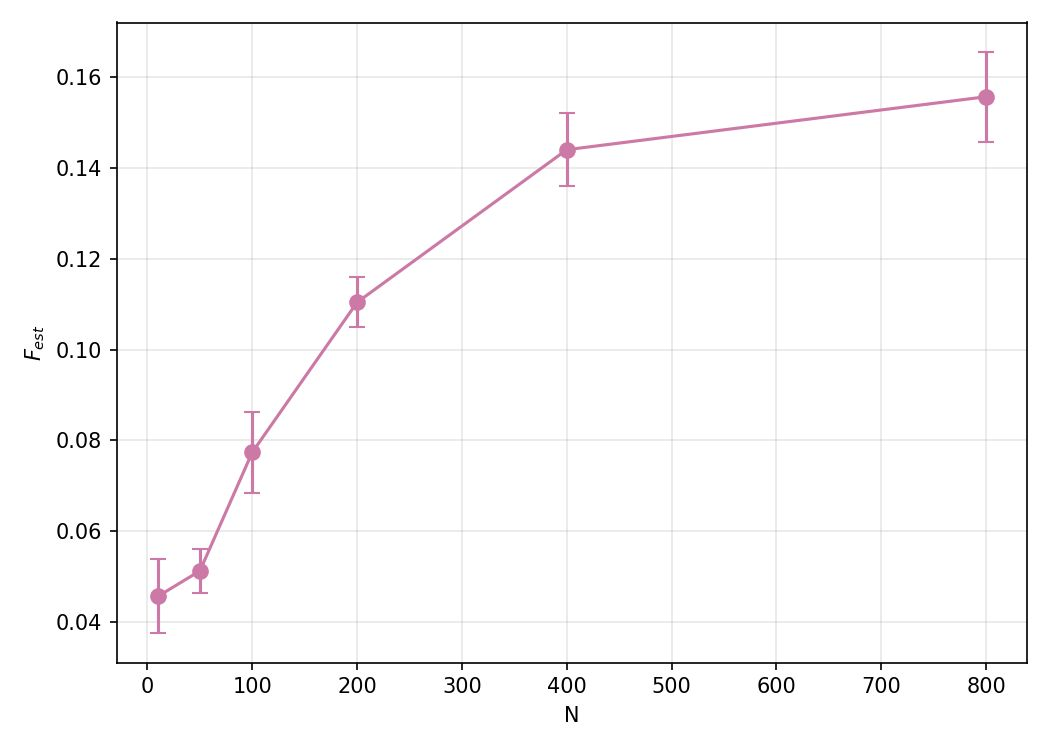
\includegraphics[width=\linewidth,height=4.5cm,keepaspectratio]{figures/graficos/1_3_Fest_vs_N.jpeg}
            \end{column}
            \begin{column}{0.5\textwidth}
                \centering
                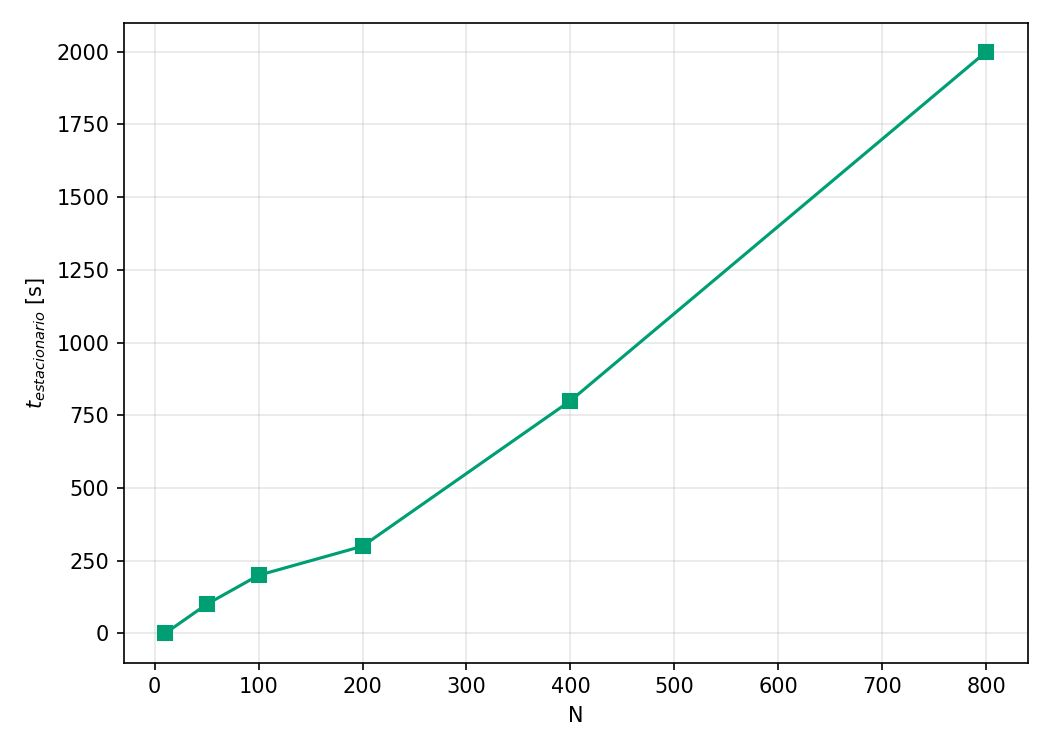
\includegraphics[width=\linewidth,height=4.5cm,keepaspectratio]{figures/graficos/1_3_tEstacionario_vs_N.jpeg}
            \end{column}
        \end{columns}
    \end{frame}

% -----------------------------------------------------------------------------
% 1.4) Perfiles radiales
% FIX punto 5: captions al pie eliminados; info trasladada al costado
% -----------------------------------------------------------------------------

    \begin{frame}{Perfiles radiales vs $S$}
        % FIX 5: el texto al pie era un caption prohibido; se mueve al costado derecho
        \begin{columns}[T]
            \begin{column}{0.98\textwidth}
                \centering
                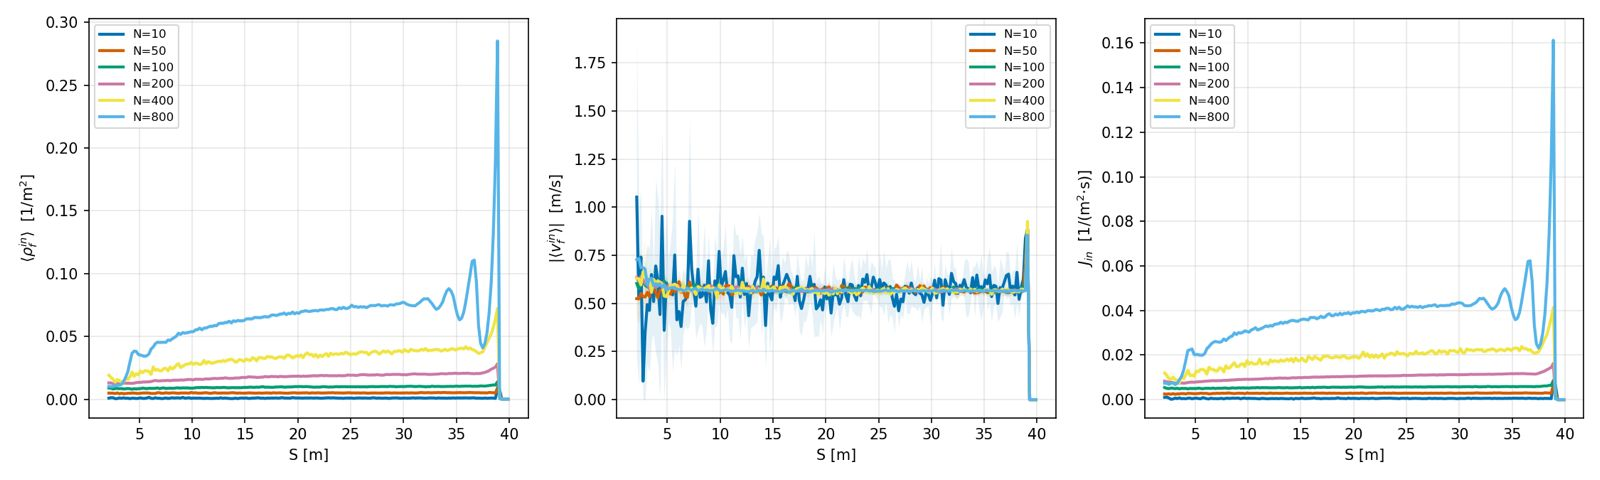
\includegraphics[width=\linewidth,height=4.5cm,keepaspectratio]{figures/graficos/1_4_perfiles_radiales.jpeg}
            \end{column}
        \end{columns}
    \end{frame}

    \begin{frame}{Observables radiales cerca de $S\!\approx\!\SI{2}{m}$ vs $N$}
        % FIX 5: el texto al pie era un caption prohibido; se mueve al costado derecho
        \begin{columns}[T]
            \begin{column}{0.98\textwidth}
                \centering
                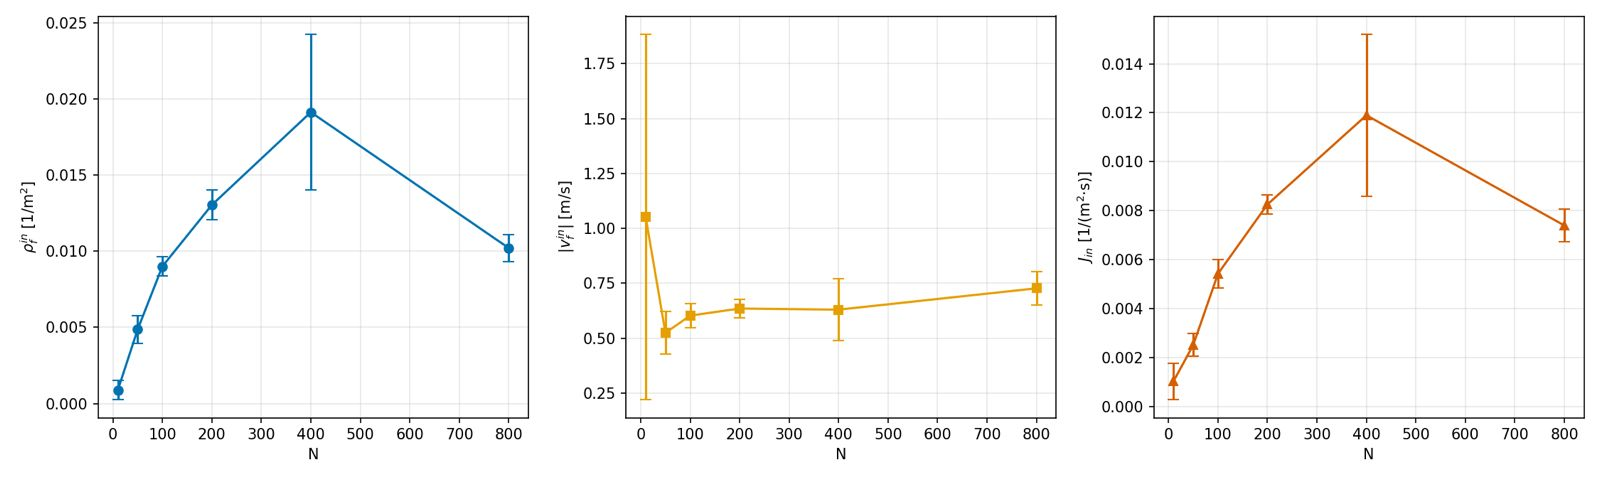
\includegraphics[width=\linewidth,height=4.5cm,keepaspectratio]{figures/graficos/1_4_observables_S2_vs_N.jpeg}
            \end{column}
        \end{columns}
    \end{frame}

% =============================================================================
% CONCLUSIONES
% FIX punto 6: solo conclusiones basadas en resultados mostrados;
%              hipótesis no probadas eliminadas; valor de N completado
% =============================================================================
    \section{Conclusiones}

    \begin{frame}[plain,c]
  \centering
  {\usebeamercolor[fg]{structure}\fontsize{48}{56}\selectfont Conclusiones\par}
    \end{frame}

    \begin{frame}{Conclusiones}
        % FIX 6: eliminada la hipótesis del "bloqueo mutuo" como conclusión autónoma
        %        (está mencionada en resultados como observación, no como conclusión independiente).
        %        El "¿DONDE?" se deja como TODO para completar con el valor real.
        %        Se eliminó cualquier referencia a cosas pendientes o descartes.
        \begin{itemize}
            \item El tiempo de ejecución crece exponencialmente con $N$ en el rango estudiado.
            \item El scanning rate $\langle J \rangle$ presenta un máximo en $N \approx 400$;
            para $N$ mayores decrece debido a la mayor fracción de partículas usadas
            acumuladas cerca del obstáculo.
            \item A mayor $N$ $\rightarrow$ Mayor $t_{\text{est}}$ y menos variable $F_{\text{est}}$.
            \item La velocidad radial $\langle v_f^{\,\text{in}} \rangle$ es aproximadamente constante 
            en todo el perfil y para todo $N \geq 50$; en consecuencia,
             $J_{\text{in}}(S)$ sigue la misma tendencia que $\langle\rho_f^{\,\text{in}}\rangle(S)$.
        \end{itemize}
    \end{frame}

% =============================================================================
% CIERRE
% =============================================================================
        {
        \setbeamertemplate{footline}{}
        \begin{frame}[plain,c]
  \centering
  {\fontsize{48}{56}\selectfont Muchas gracias\par}
        \end{frame}
    }

\end{document}